%% F2
\begin{figure*}[ht]
  \begin{subfigure}{.315\textwidth}
    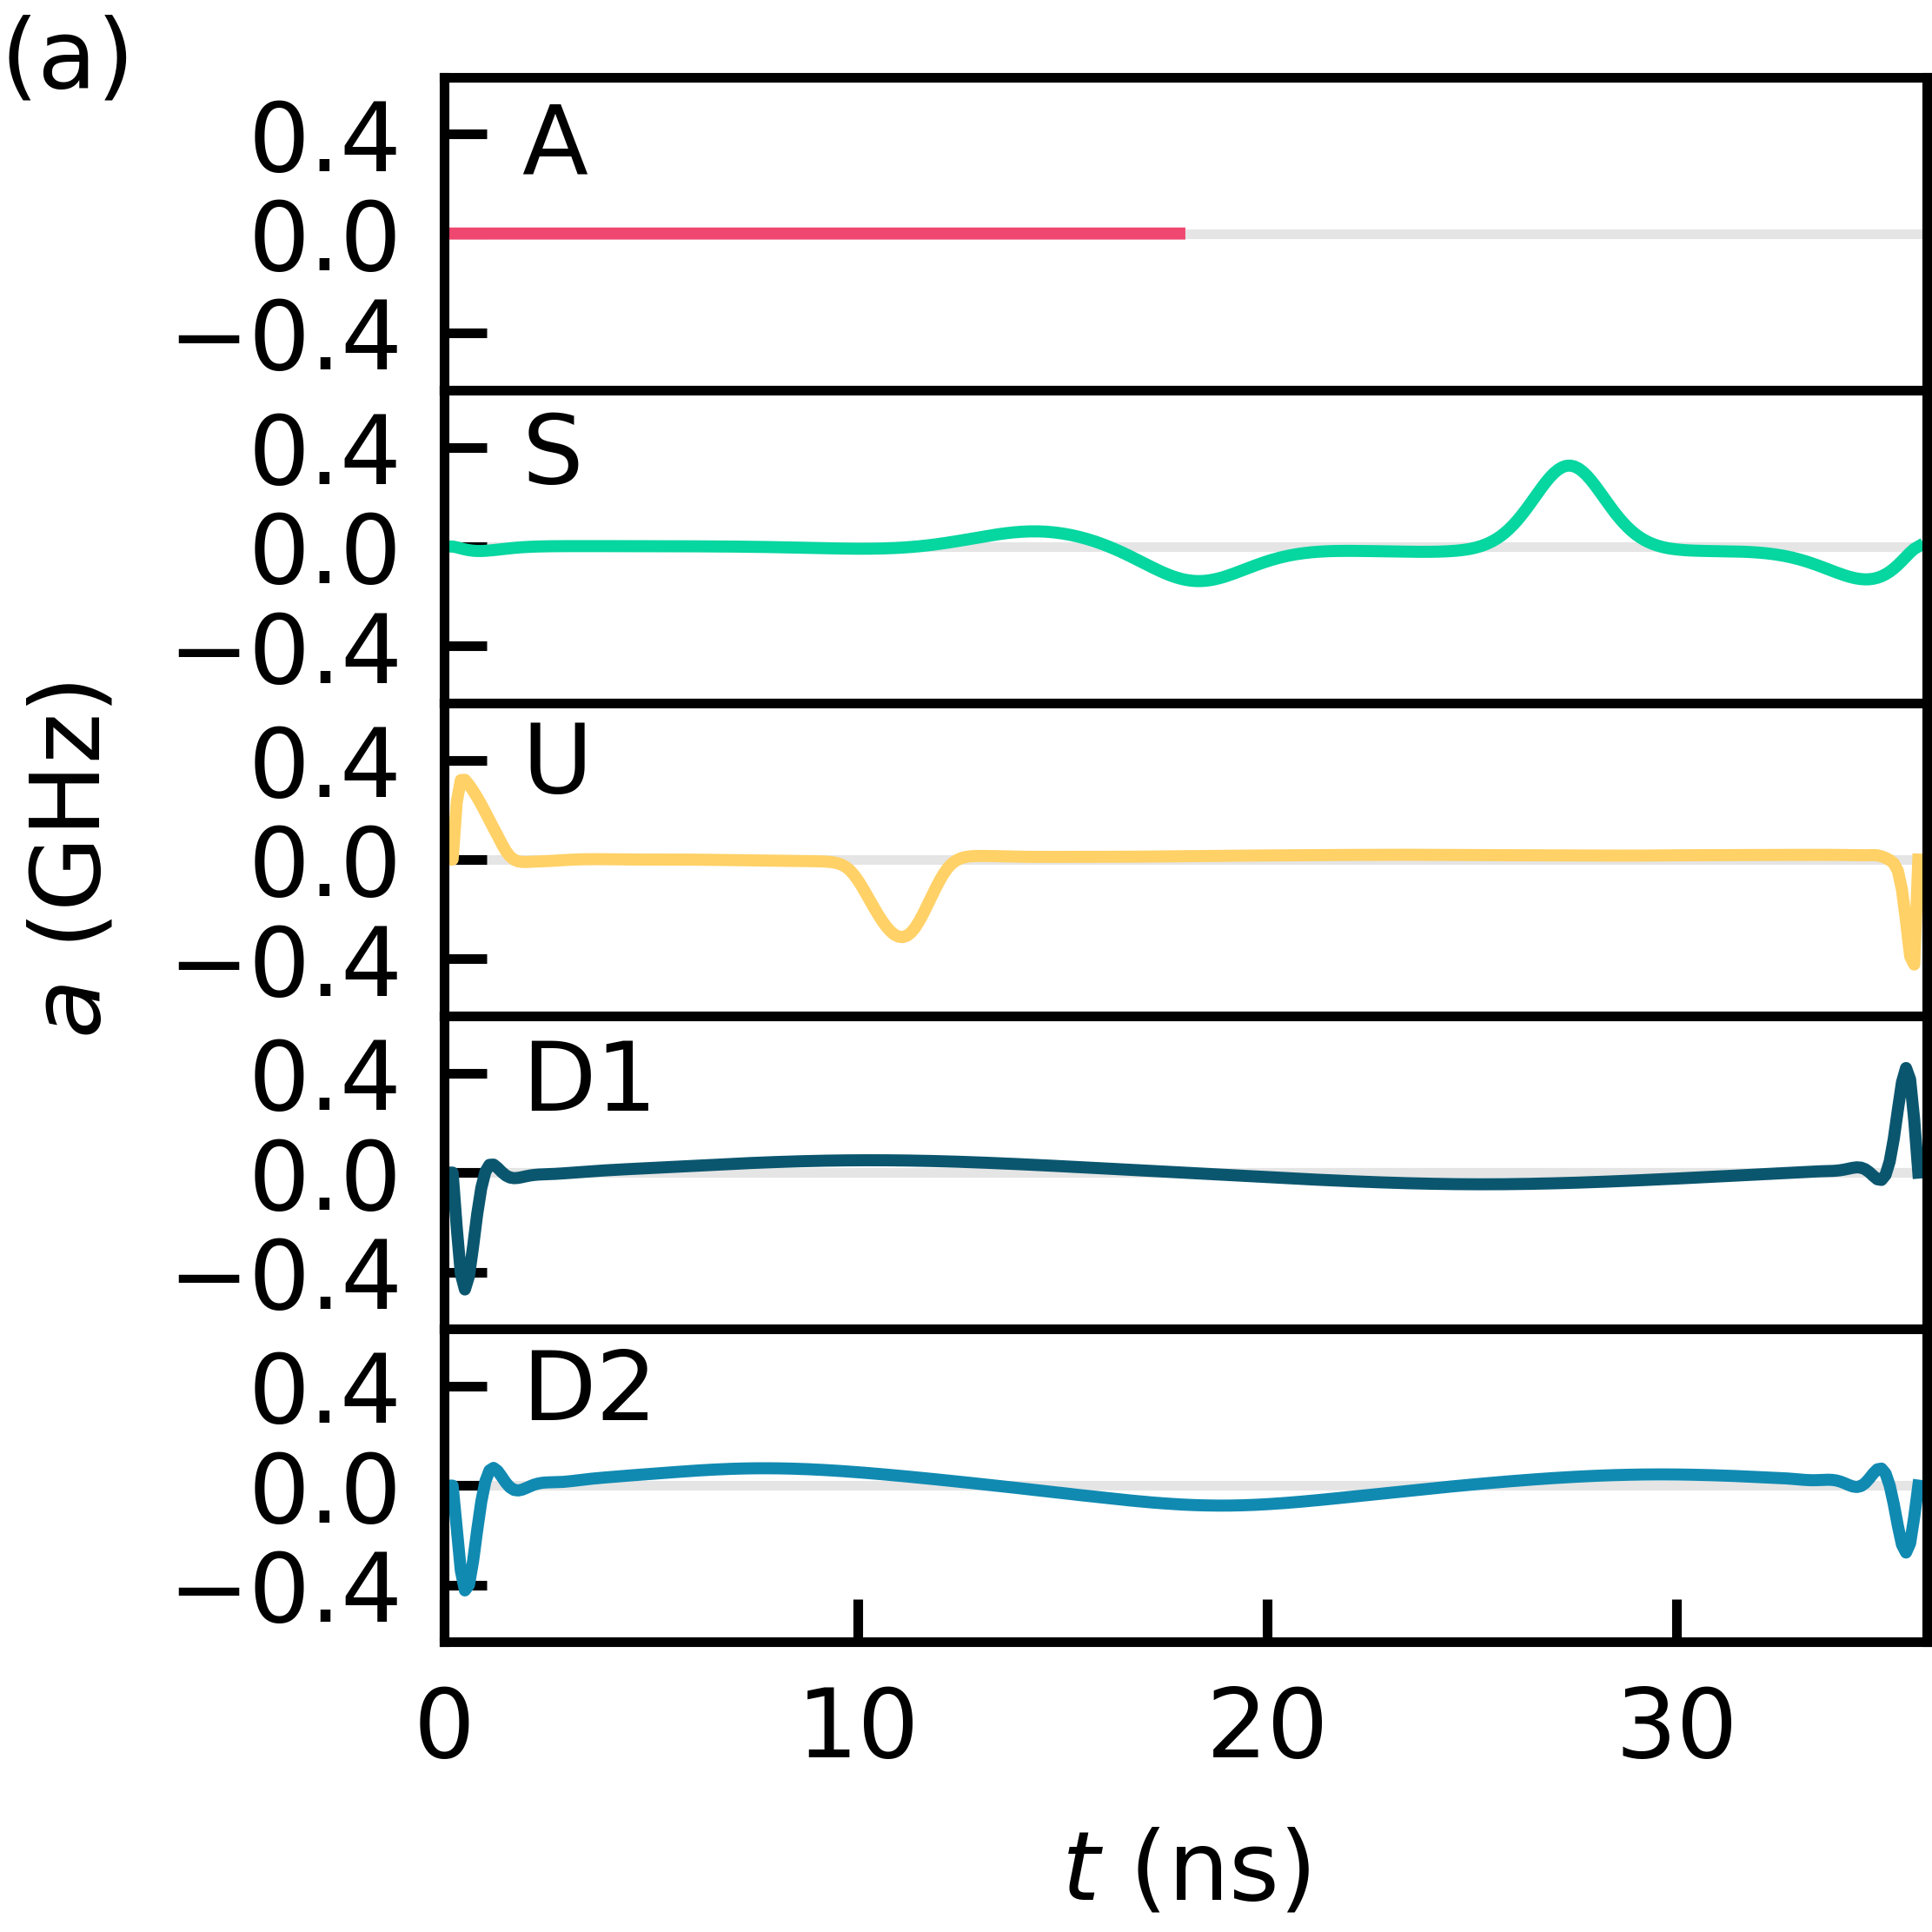
\includegraphics[width=\linewidth]{assets/f2a.png}
    \caption{\label{fig:statica}}
  \end{subfigure}\hfill
  \begin{subfigure}{.4\textwidth}
    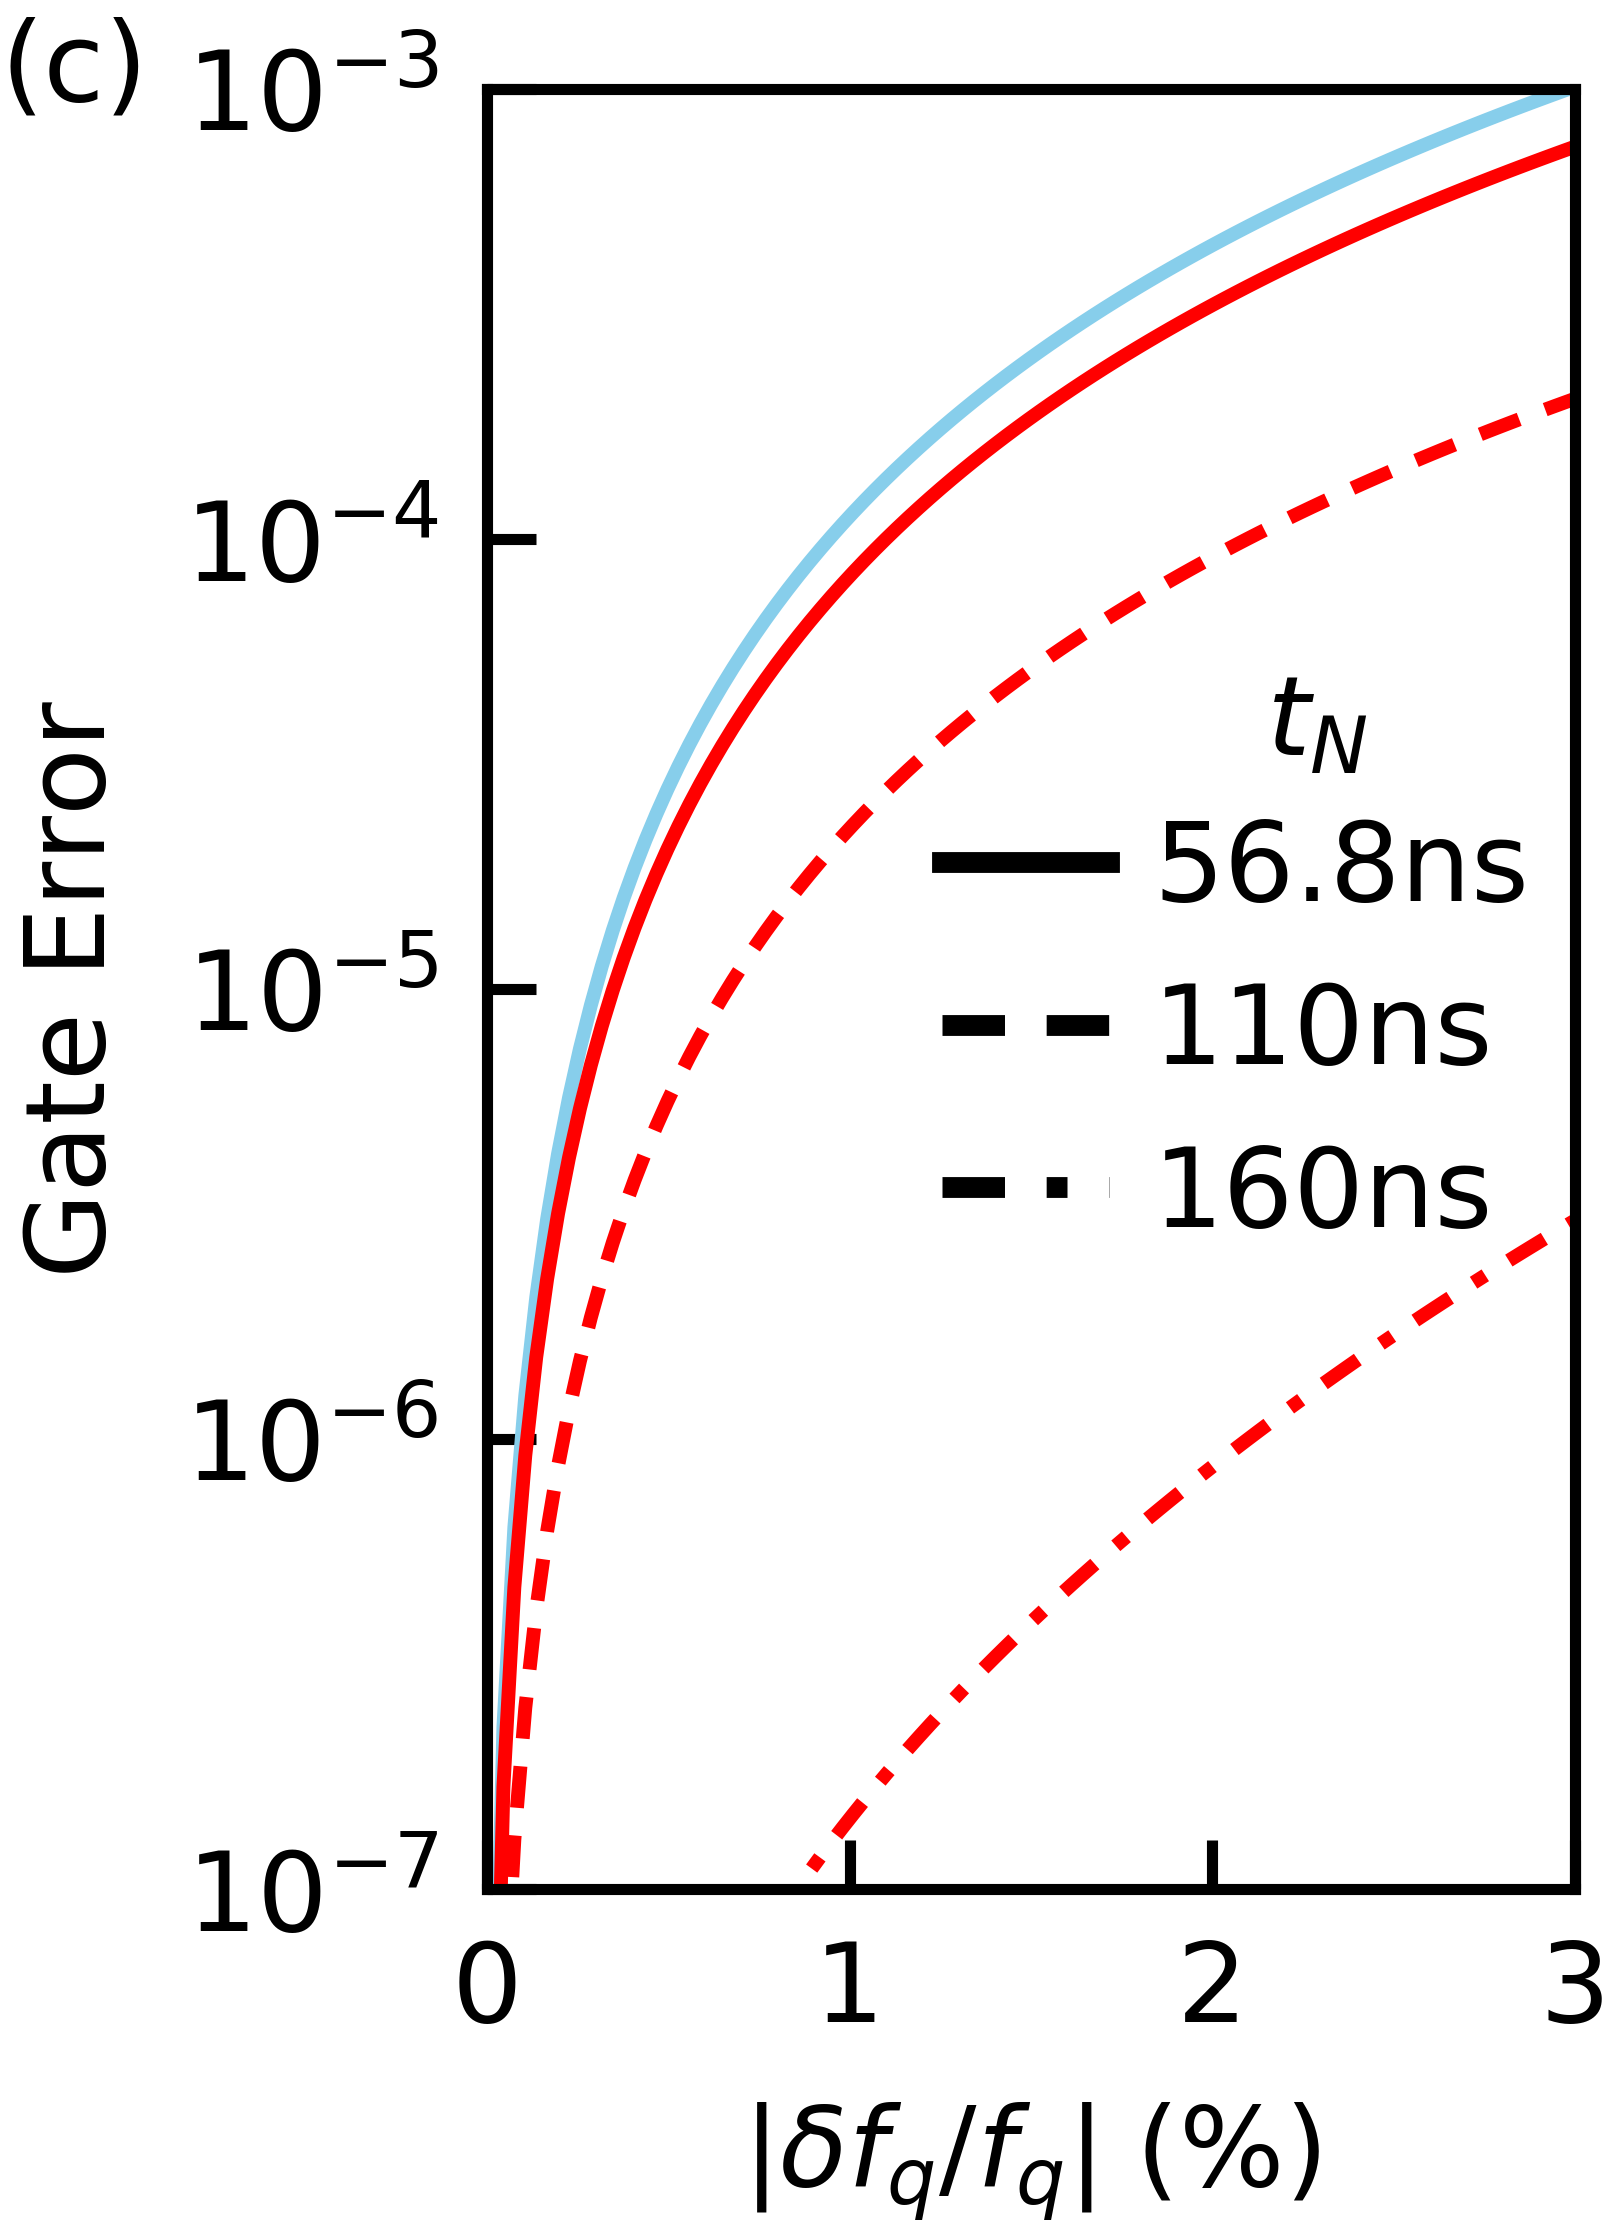
\includegraphics[width=\linewidth]{assets/f2b.png}
    \caption{\label{fig:staticb}}
  \end{subfigure}\hfill
  \begin{subfigure}{.23\textwidth}
    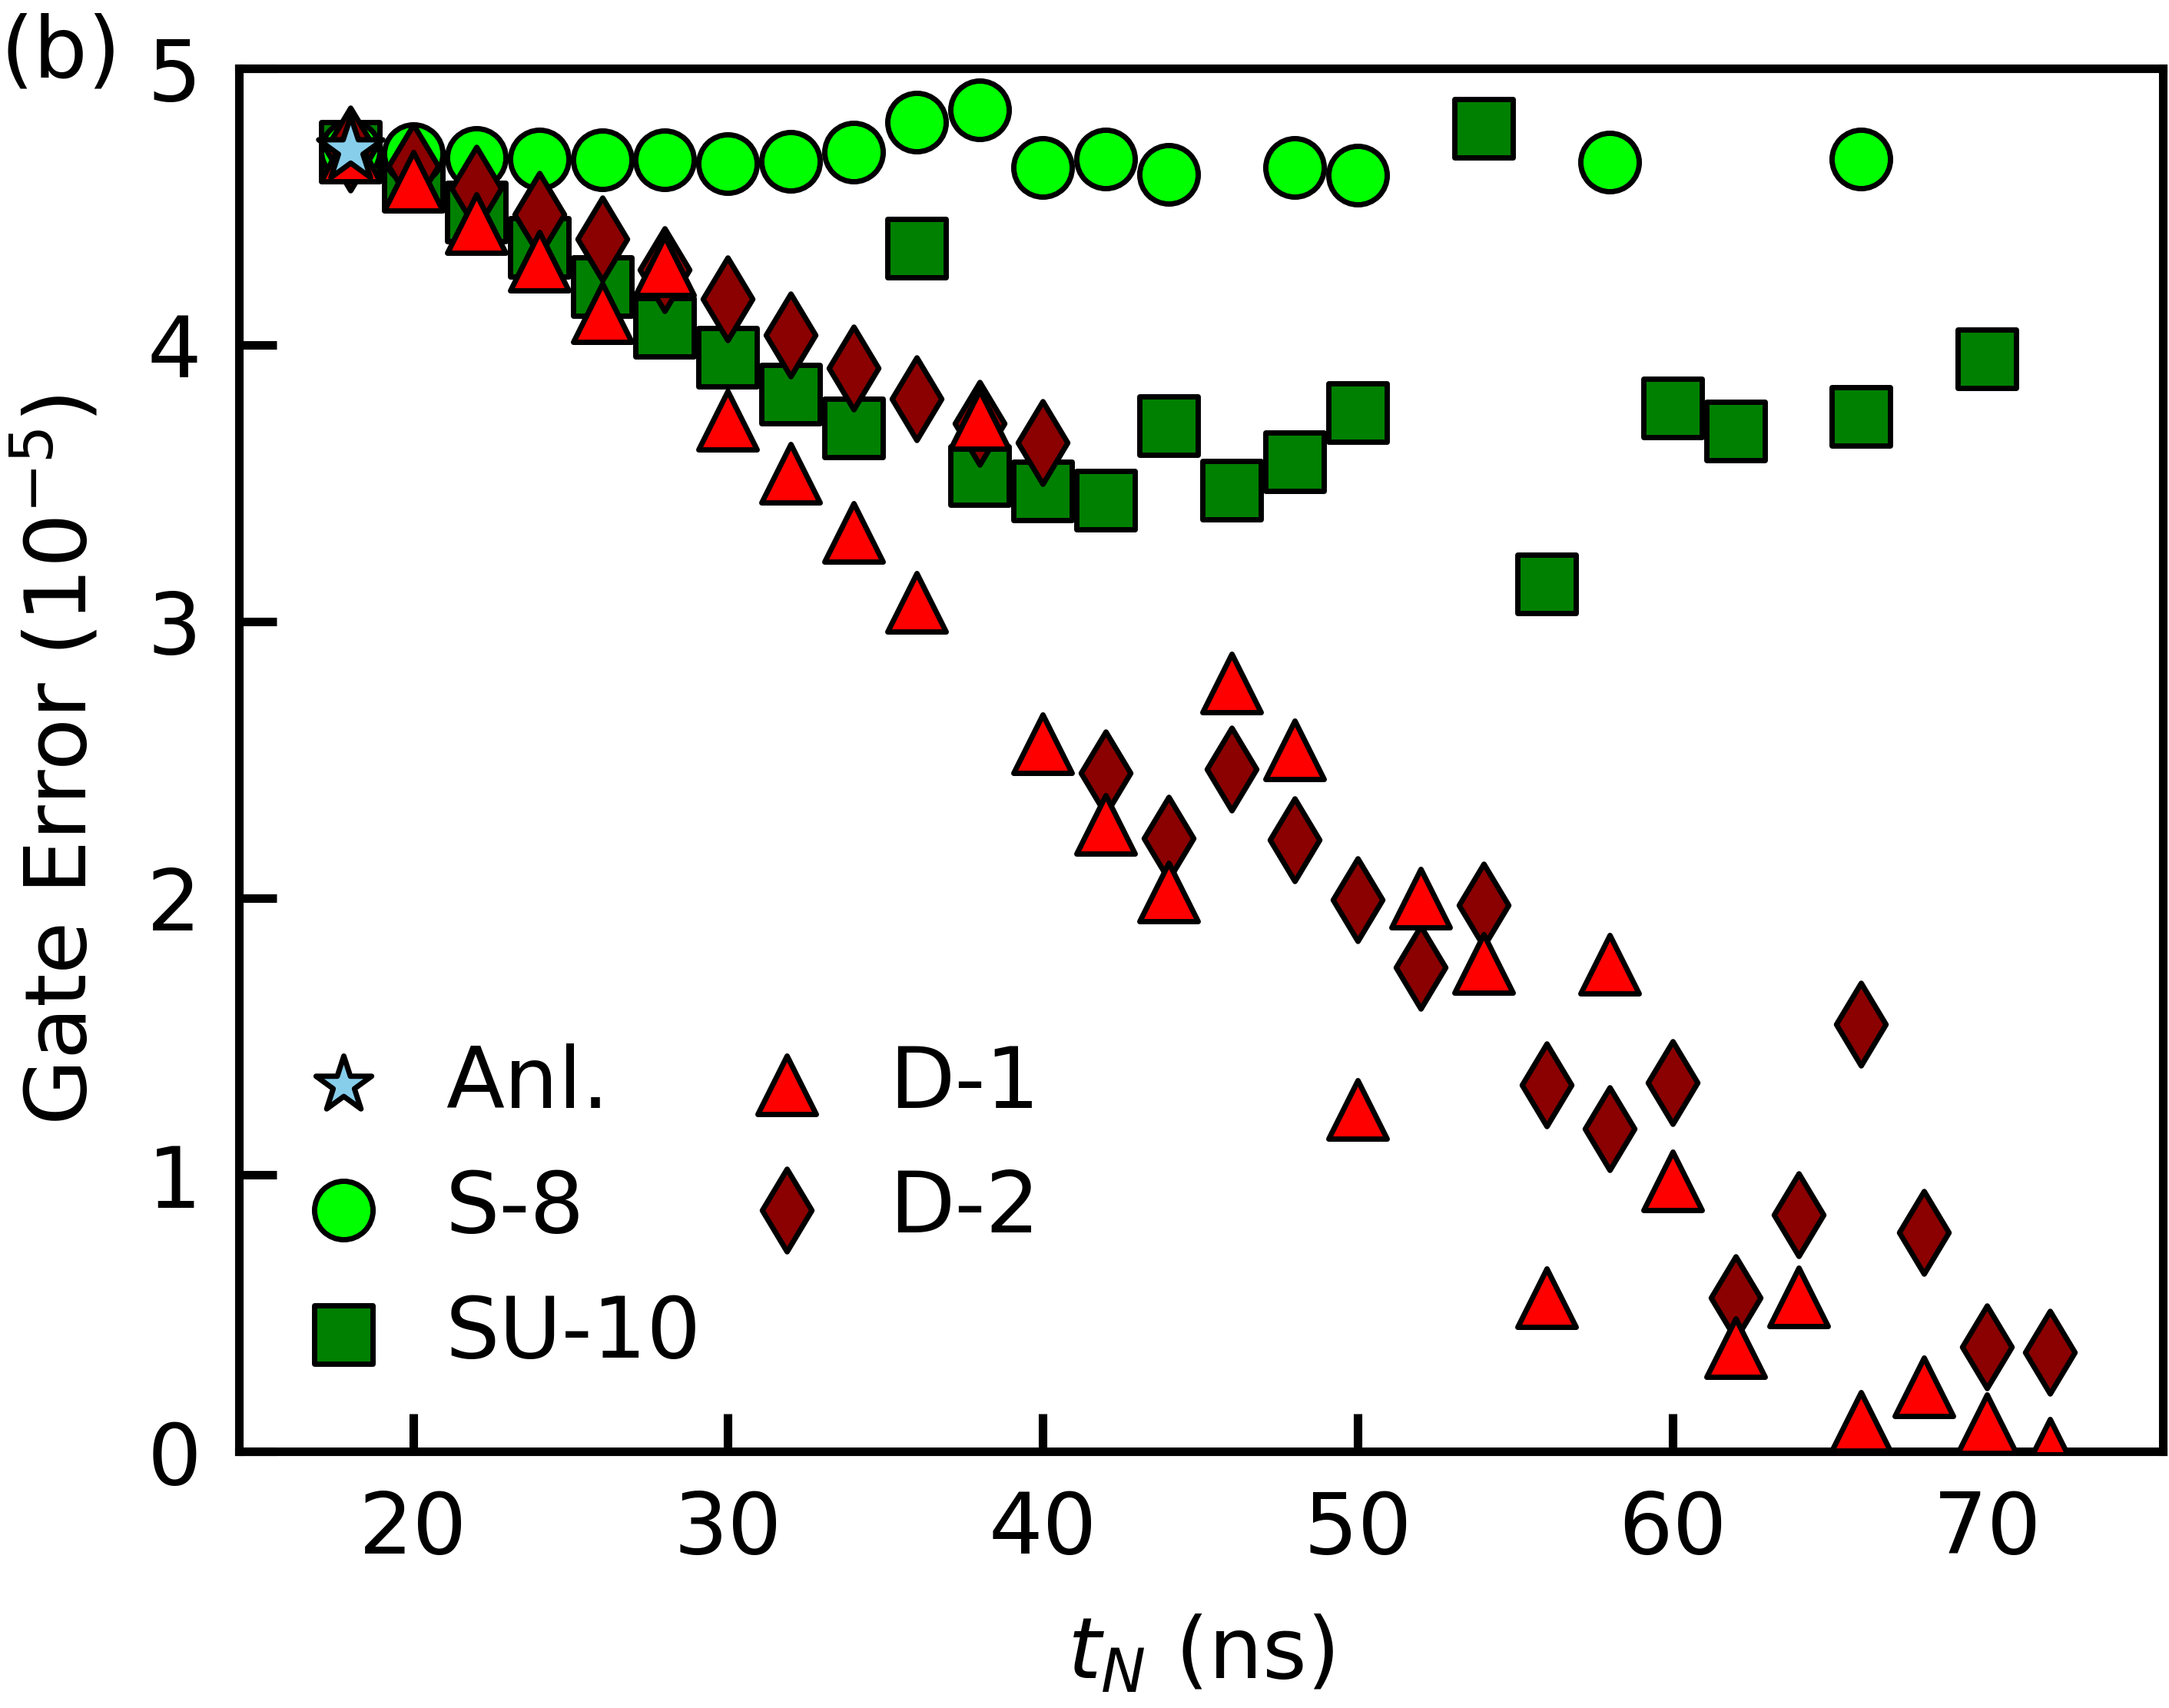
\includegraphics[width=\linewidth]{assets/f2c.png}
    \caption{\label{fig:staticc}}
  \end{subfigure}
  \caption{
    (a) Flux pulses for $Z/2$ gates robust to qubit frequency detunings constructed with the
    analytic (A), sampling (S), unscented sampling (U), and the 1\textsuperscript{st}-
    and 2\textsuperscript{nd}-order derivative methods (D1, D2). The flux pulses shown
    for the sampling, unscented sampling, and derivative methods are optimized
    for twice the gate time of the analytic gate.
    (b) Single gate error at a one-percent qubit frequency detuning as
    a function of the gate time. Missing
    data points represent gates with a gate error greater than $5 \cdot 10^{-5}$
    \todo{...what's going on here? Should I be concerned? This seems like a relatively big thing that goes unexplained}.
    (c) Single gate error as a function of the qubit frequency detuning.
    The gate errors for the analytic and 1\textsuperscript{st}-order derivative
    methods are shown for gate times which are multiples of $1 / 4 f_{q} \sim 18 \textrm{ns}$.
    The gate errors for the two methods are
    indistinguishable at the gate time $18 \textrm{ns}$.
  }
  \label{fig:static}
\end{figure*}

\section{Robustness to Static Parameter Uncertainty \label{sec:static}}
We have formulated the QOC
problem as an open-loop optimization problem; equivalently,
we do not incorporate feedback from the experiment in optimization.
However, the device's parameters deviate from the parameters we use in optimization,
leading to poor experimental performance. We combat errors
of this form using robust control techniques,
making the state evolution insensitive
to parameter uncertainty. As an example,
we mitigate errors arising from the drift and finite measurement
precision of the qubit frequency which modifies the fluxonium Hamiltonian
\eqref{eq:hamiltonian} by $f_{q} \rightarrow f_{q} + \delta f_{q}$.
We consider three robust control techniques to accomplish this task:
a sampling method, an unscented sampling method,
and a derivative method.

The sampling method incentivizes the optimizer
to ensure multiple copies of a state, each of which evolves
with a distinct value of the uncertain parameter, achieve
the same target state. Variants of this technique have been proposed
in the context of QOC
\cite{allen2019robust, ball2020software, khaneja2005optimal,
  reinhold2019controlling, rembold2020introduction} and applied
experimentally \cite{carvalho2020error}.
For each initial state,
we add two sample states $\ket{\psi^{\pm}}$
to the augmented state \eqref{eq:astatecontrols}. The discrete dynamics
function \eqref{eq:dyn_con} is modified
so the sample states evolve under the fluxonium Hamiltonian \eqref{eq:hamiltonian}
with $f_{q} \rightarrow f_{q} \pm \sigma_{f_{q}}$ for a fixed
hyperparameter $\sigma_{f_{q}}$ which is the standard deviation of the qubit frequency.
We penalize the infidelities of the sample states and their target state
by adding a cost function to the objective \eqref{eq:costfun} of the form
$\sum_{k, \pm} b_{k} (1 - {\lvert \bra*{\psi^{\pm}_{k}}U\ket*{\psi_{1}} \rvert}^{2})$
where $b_{k}$ is a constant we supply.
\todo{I thought of this question here but it applies also to when we first write down the objective 6a.
Doesn't the sum over k imply that we are penalizing the time it takes to complete the gate?
Why do we need to append $\Delta t_{k}$ to the augmented state vector?}
For this method, the standard orthonormal basis states are an insufficient choice
for the initial states. As an example, a $Z/2$ gate achieved by idling
at the flux frustration point $a_{k} = 0 \ \forall \ k$
will be robust to qubit frequency detunings for the initial states $\ket{0}$
or $\ket{1}$ because the infidelity metric is insensitive to global phases,
but this gate will not be robust for any other initial states.
Therefore, we choose four initial states
so that their outer products
span the operators on the Hilbert space
$\{\ket{0}, \ket{1}, (\ket{0} + i\ket{1}) / \sqrt{2},
(\ket{0} - \ket{1}) / \sqrt{2}\}$ \cite{chow2009randomized},
which we refer to as the operator basis.

Whereas the sampling method penalizes the deviations of the sample states
from the target state, the unscented sampling method
penalizes the deviations of the sample states from the nominal state
\cite{howell2020direct, lee2013sigma,
  thangavel2020robust}. Accordingly, the cost function we add
to the objective \eqref{eq:costfun} takes the form
$\sum_{k, j} c_{k} (\psi^{j}_{k} - \psi_{k})^{T}
(\psi^{j}_{k} - \psi_{k})$, where $c_{k}$ is a
constant we supply, $\psi_{k}$ is
the evolved initial state (nominal state), and $\psi^{j}_{k}$ is a sample state
that evolves under a modified Hamiltonian similar to that in the sampling method.
We omit bra-ket notation here to emphasize that
the states are real vectors, and are given by the right-hand-side of the
isomorphism \eqref{eq:isomorphism}. Additionally,
the unscented sampling method employs the unscented transform
\cite{julier2004unscented, uhlmann1995dynamic}
to prevent the sample states
from drifting too far or close to the nominal state during evolution,
which would result in exceedingly large or small deviations in the cost function.
In particular, the sample states are chosen to encode a unimodal distribution over
the $2n$ \todo{at this point the reader has forgotten what lower-case n refers to} elements of the nominal state, modeling the uncertainty in the state
as a result of the uncertainty in the parameter. The unscented transform
accurately propagates the mean and covariance of this distribution between
knot points, or equivalently, through the transformation of the TDSE.
For this method, we sample on one initial state $(\ket{0} + i\ket{1}) / \sqrt{2}$,
and do not observe a performance increase
using more initial states, for example those from the operator basis.
A detailed procedure for the unscented transformation is given
in Appendix \ref{appendix:unscented}.
\todo{this seems far more complicated than the sampling method - if it truly is necessary,
  perhaps earlier we could fully flesh out what the issues are?
  Does this drifting too close to the nominal state actually occur in practice?
  And if so, it isn't clear to me why that is a bad thing, as for example if it drifts close to the nominal state,
  then great, isn't the optimizer doing its job?}

The derivative method penalizes the sensitivity of the state
to the uncertain parameter, which is encoded in the $l$\textsuperscript{th}-order
state derivative $\partial_{f_{q}}^{l} \ket{\psi}$ \todo{seems funny to change from $l$ to $m$ immediately after introduction}.
In the $m$\textsuperscript{th}-order
derivative method, we append all state derivatives of order $1, \dots, m$
to the augmented state vector \eqref{eq:astatecontrols}
for each initial state. We use the initial state $\ket{0}$ for this method,
and observe no advantage to using more initial states
\todo{comment on why you've chosen different states for this vs. unscented?}.
We penalize the norms of the state derivatives
in the objective \eqref{eq:costfun} by setting the corresponding elements
of the final augmented state to zero
\todo{this isn't totally obvious to me - why should this be the right way to penalize?
  Also the wording seems a bit off - surely you don't mean that you're penalizing the norm of the state derivative with itself? Isn't it normalized?}.
We could obtain the state derivatives at each knot point
with backward-mode differentiation.
In a naive automatic differentiation scheme,
the discrete dynamics function at knot points
$1, \dots, k - 1$ would be differentiated to obtain the state
derivative at knot point $k$, requiring
$O(N^{2})$ matrix multiplications. Instead, we 
employ forward-mode differentiation on the TDSE \eqref{eq:tdse}
to obtain coupled, first-order ODEs
which require $O(N)$ matrix multiplications to integrate.
For example, the dynamics for the $1$\textsuperscript{st}-order derivative method are:
\begin{align}
  i \hbar \frac{d}{dt} \ket{\psi} &= H \ket{\psi},\\
  i \hbar \frac{d}{dt} \ket{\partial_{f_{q}}\psi} &=
  H \ket{\partial_{f_{q}} \psi} +
  (\partial_{f_{q}} H) \ket{\psi}.
  \label{eq:d1dyn}
\end{align}
We integrate the coupled ODEs with exponential
integrators
in the discrete dynamics function \eqref{eq:dyn_con}, see Appendix \ref{appendix:derivative}.
For runtimes
of the three robust control techniques,
consult Appendix \ref{appendix:time}.

\todo{you have obviously made the choice to first present all three methods as theoretical tools,
  then discuss their results together, which is fine. It might make sense to also consider presenting
  a method and presenting results associated with that method, before moving on to the next one.
  Might make it easier to justify, e.g., the complexity of the unscented sampling method
  if there are deficiencies to be addressed that are clear from the results of the sampling method.}
We examine the gate errors due to a static qubit frequency
detuning for the $Z/2$ gates obtained with the robust control techniques
and the analytic $Z/2$ gate.
To compute the gate error,
an initial state is evolved
under the fluxonium Hamiltonian \eqref{eq:hamiltonian}
two separate times with the transformations
$f_{q} \rightarrow f_{q} \pm \delta f_{q}$
at the stated qubit frequency detuning $\delta f_{q}$.
The reported gate error is the infidelity of
the evolved state and the target state averaged over
the two transformations for each of $1000$ pseudorandomly
generated initial states.
We set $\sigma_{f_{q}}/f_{q} = 1\%$
for the sampling and unscented sampling
methods.
\todo{right so reading further - this paragraph has nothing to do with the previous two
  - might make sense to put this with the corresponding explanation of the method.}

The analytic gate corresponds to
idling at the flux frustration point $a_{k} = 0 \ \forall \ k$, see Figure
\ref{fig:statica}. Its gate time $1 / 4 f_{q} \sim 18\textrm{ns}$
is the shortest possible for a $Z/2$ gate on the device.
The gate's erroneous rotation angle
$2 \pi \delta f_{q} / 4 f_{q}$ is linear in the
qubit frequency detuning, resulting in a gate error that is quadratic
in the detuning.
At a one-percent
detuning ($\lvert \delta f_{q} \rvert / f_{q} = 1\%$),
the gate error is $\sim 4.5 \cdot 10^{-5}$,
which is sufficient for quantum error correction.
Although the gate performs well, it cannot be extended
to gate times other than
$1 / 4 f_{q}$. The ability to perform
phase gates in any given time is critical
for multi-qubit experiments, where the qubits operate at different
frequencies.
We can find solutions using the numerical methods at
all gate times above $18$ns, see Figure \ref{fig:staticb}.
These numerical methods offer an effective scheme for synchronizing
multi-qubit experiments.
\todo{this seems like a funny way to end this paragraph - I was told that static parameter deviations were the issue the whole time, and suddenly it's that analytic pulses aren't flexible enough w.r.t. the time it takes to complete them. I would stress instead that you can do better than $\sim 4.5 \cdot 10^{-5}$! The time issue, though important, feels like it should be more of an aside given the things you've emphasized are the issues you're trying to solve.}

The flux pulse produced by the sampling method
transitions  smoothly away from idles at the flux frustration point,
whereas that for the unscented sampling method employs
three distinct transitions.
The gate error at a one-percent qubit frequency detuning for the sampling method
does not improve substantially over the
range of gate times. Conversely, the gate error at a one-percent detuning
for the unscented sampling method reaches a minimum of $\sim 3.9 \cdot 10^{-5}$
near fractions of the Larmor period $2/4f_{q} \sim 36\textrm{ns},
3/4f_{q} \sim 54\textrm{ns}, 4/4f_{q} \sim 72\textrm{ns}$.

The two derivative methods converge on qualitatively similar flux pulses that
use fast triangle pulses at the boundaries and idle near the flux frustration point,
similar to the flux pulse produced by the unscented sampling method.
The gate errors at a one-percent qubit frequency detuning
for both derivative methods decrease super-linearly in their gate times.
The 2\textsuperscript{nd}-order method does not offer a substantial improvement
over the 1\textsuperscript{st}-order method for most gate times.
\todo{I would say the second order method as compared to the first order method feels the same as the sampling method as compared
  to the unscented method. You say here that there is no improvement, but improvement for unscented looks mostly like noise to me,
  even if you have some idea of where it's coming from (larmor period fractions).
  I would just be careful with how these things are framed - seems opportunistic to claim that unscented gives some sort of serious advantage here.}
The gate error at a one-percent detuning for the 1\textsuperscript{st}-order
method reaches $10^{-7}$ at the Larmor period $1 / f_{q} \sim 72$ns,
see Figure \ref{fig:staticc}.
This result mimics the
ability of composite pulses to mitigate parameter uncertainty errors to arbitrary
order with sufficiently many pulses \cite{merrill2014progress}.
It is difficult to choose an appropriate composite pulse
for the problem studied here due to our Hamiltonian and experimental constraints.
We propose comparisons between composite pulses and numerical techniques
for future work.

%% F3
\begin{figure*}[ht]
  \begin{subfigure}{.4\textwidth}
    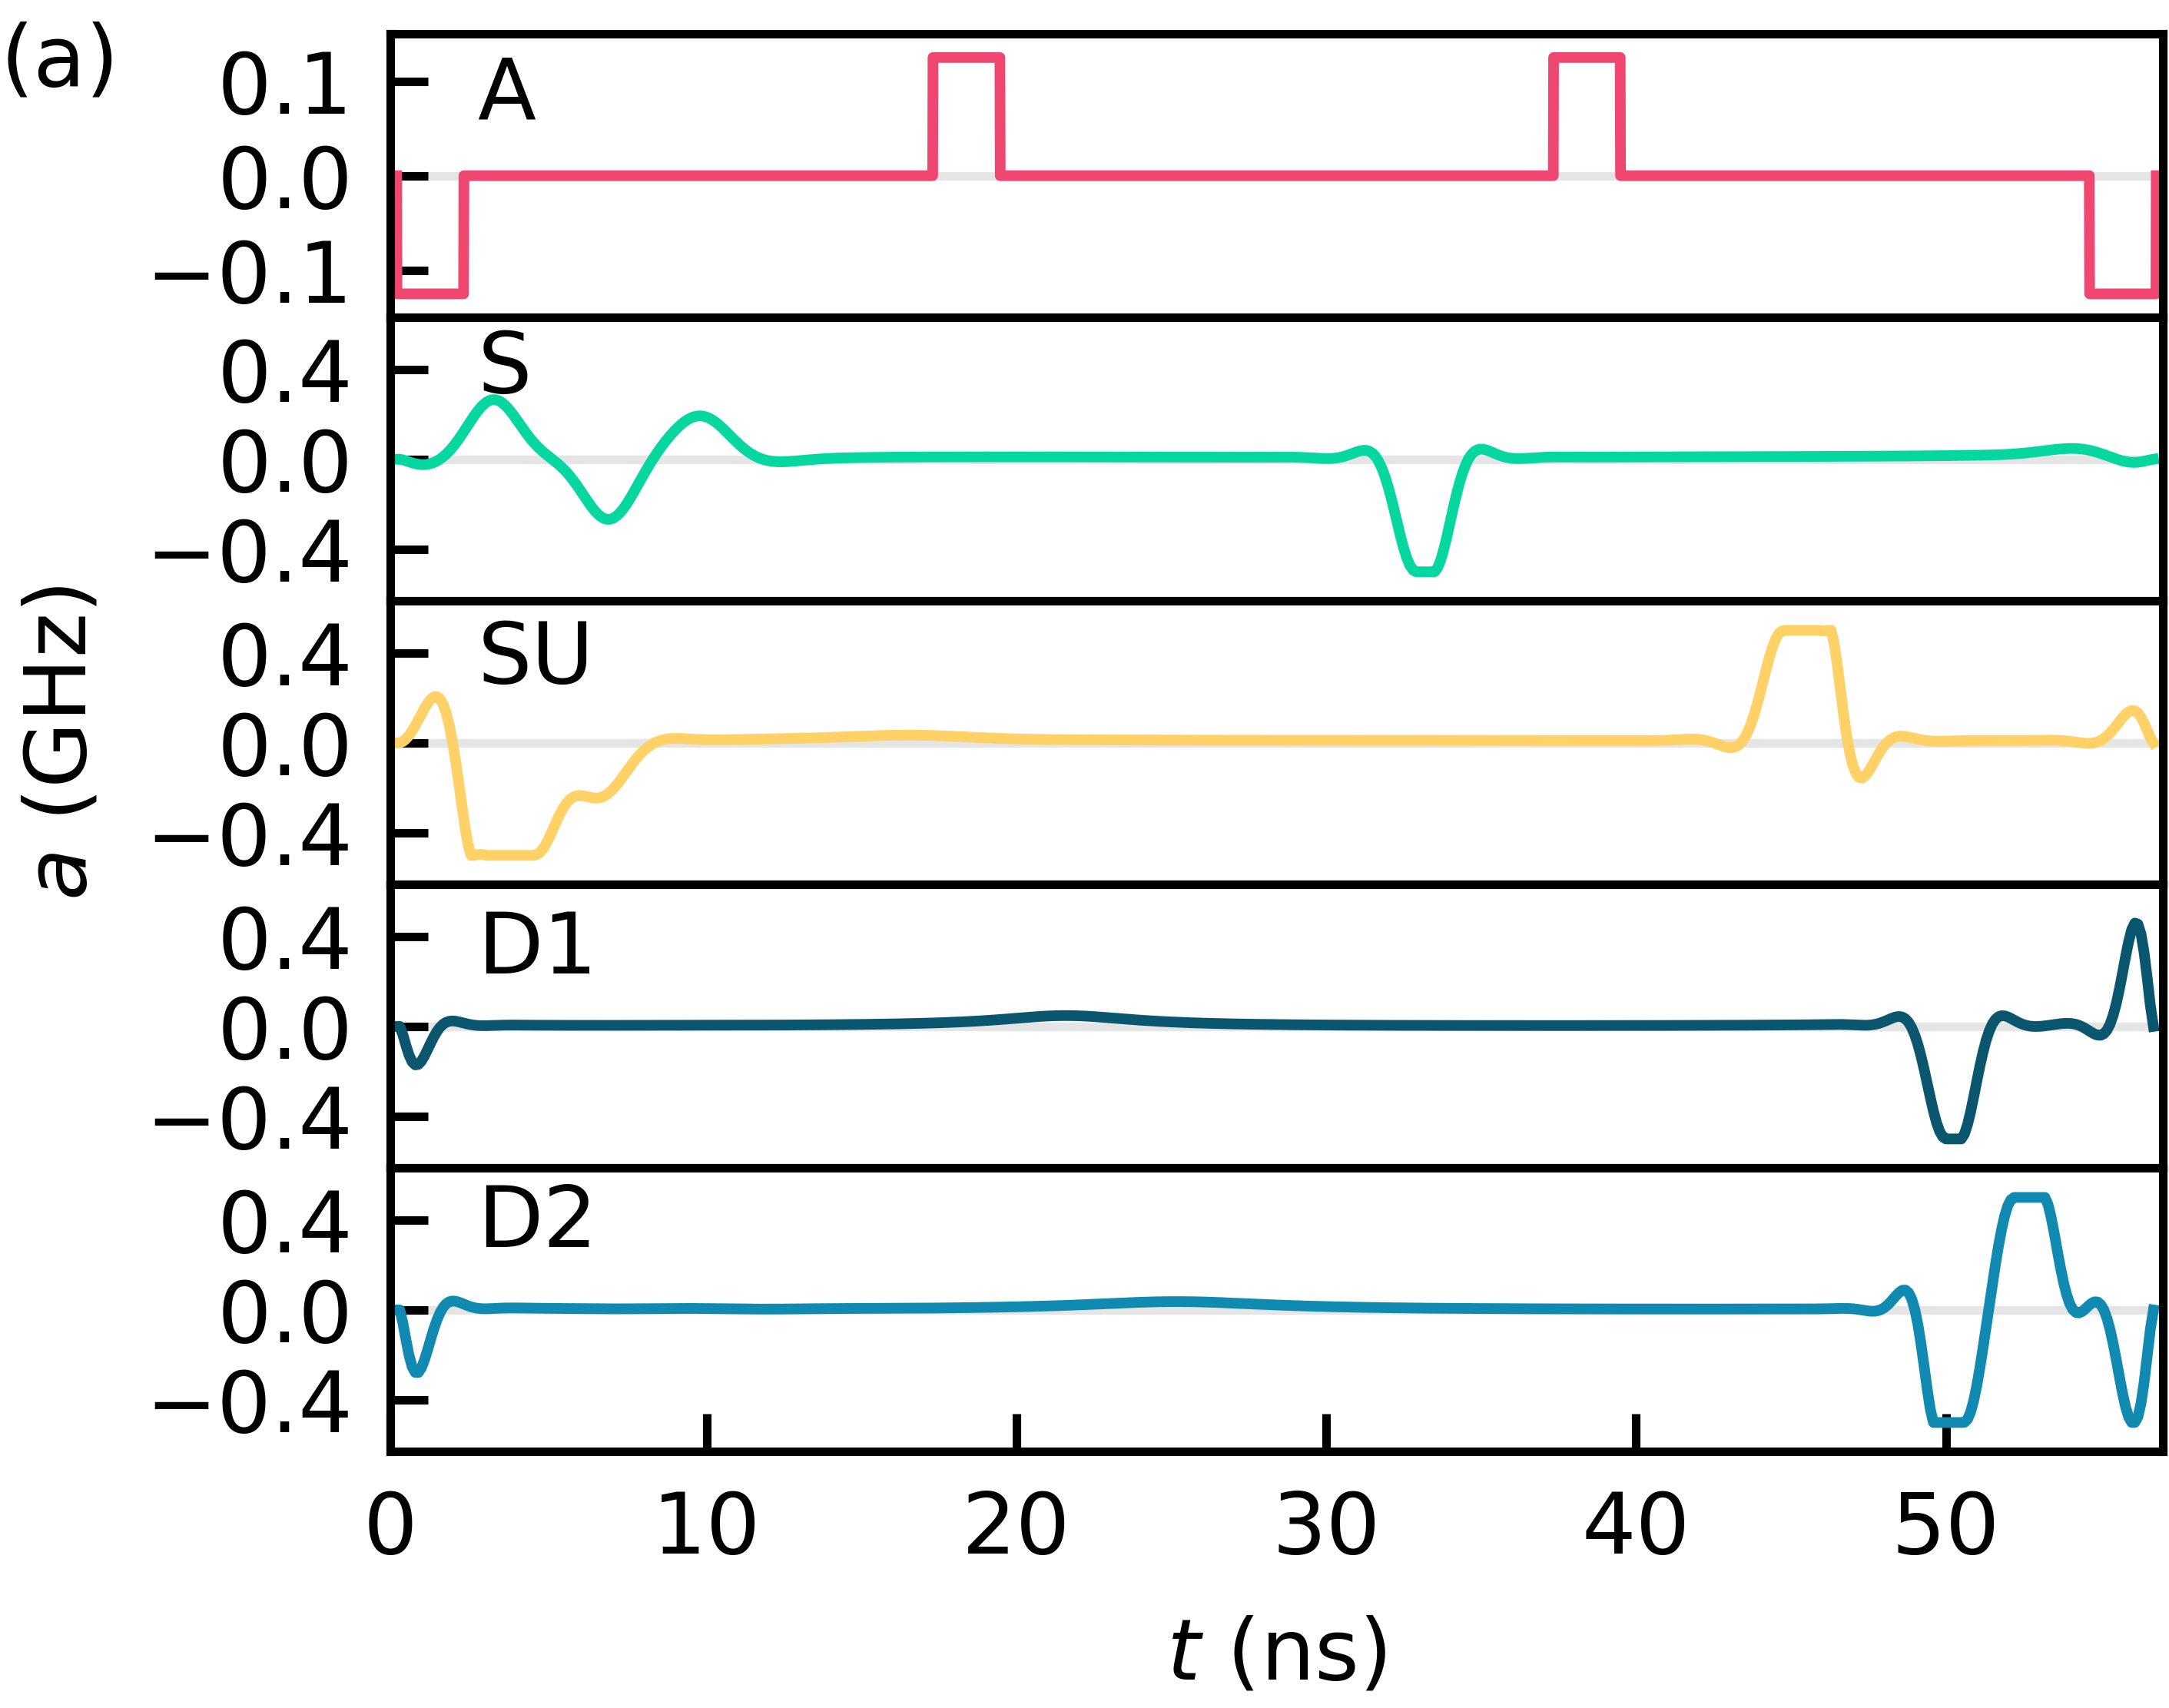
\includegraphics[width=\linewidth]{assets/f3a.png}
    \caption{}
    \label{fig:stochastica}
  \end{subfigure}\hspace{0.05\textwidth}
  \begin{subfigure}{.4\textwidth}
    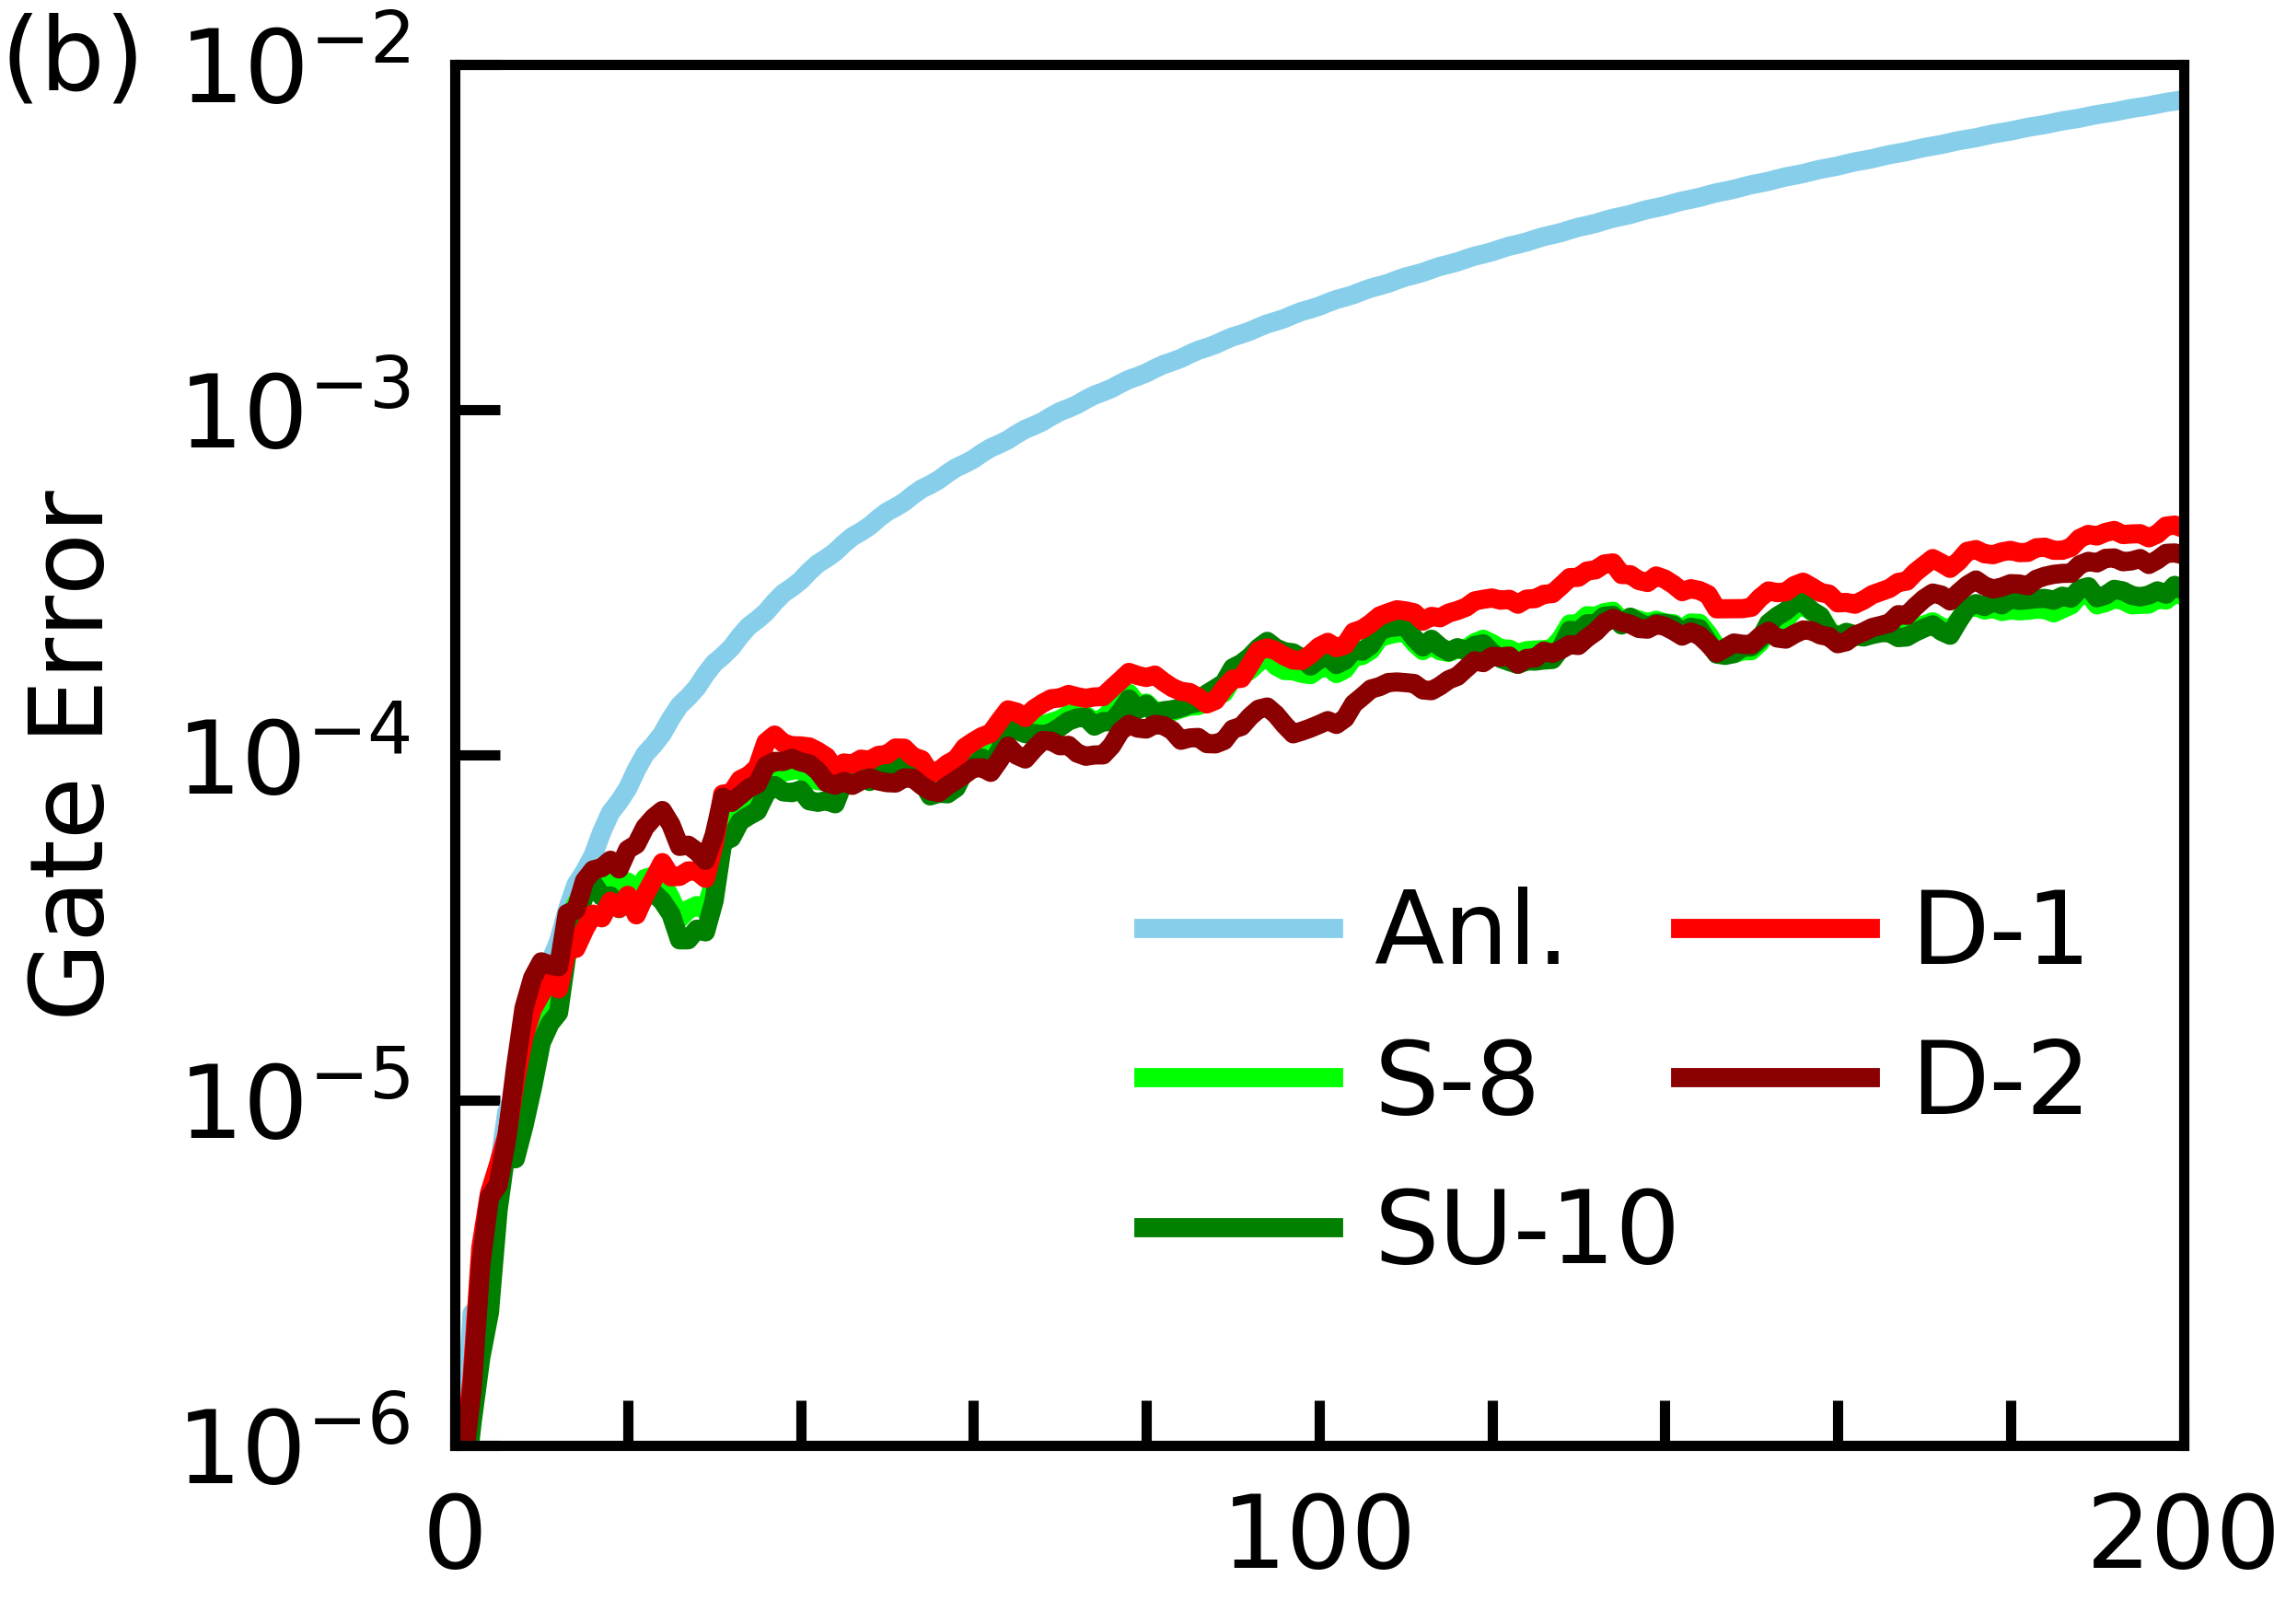
\includegraphics[width=\linewidth]{assets/f3b.png}
        \caption{}
    \label{fig:stochasticb}
  \end{subfigure}
  \caption{
    (a) Flux pulses for $X/2$ gates robust to flux offsets
    constructed with the analytic (A),
    sampling (S), unscented sampling (U), and the 1\textsuperscript{st}-
    and 2\textsuperscript{nd}-order derivative methods (D1, D2).
    (b) Cumulative gate error due to 1/$f$ flux noise for
    successive gate applications. The cumulative gate errors for the
    sampling, unscented sampling, and the derivative methods are indistinguishable.
  }
  \label{fig:stochastic}
\end{figure*}
